\hypertarget{commercially-usable-data-sets}{%
\section{Appendix D: Commercially-usable datasets}\label{commercially-usable-data-sets}}

\hypertarget{data-vendors}{%
\subsection{Data vendors}\label{data-vendors}}

Both platforms below provide similar corpora in different languages,
both provide data for ASR and face tracking
\href{http://catalogue.elra.info/en-us/}{European language resource
association}

\href{http://www.d-ear.com/CCC/corpora.htm}{Chinese Corpus Consortium} \\
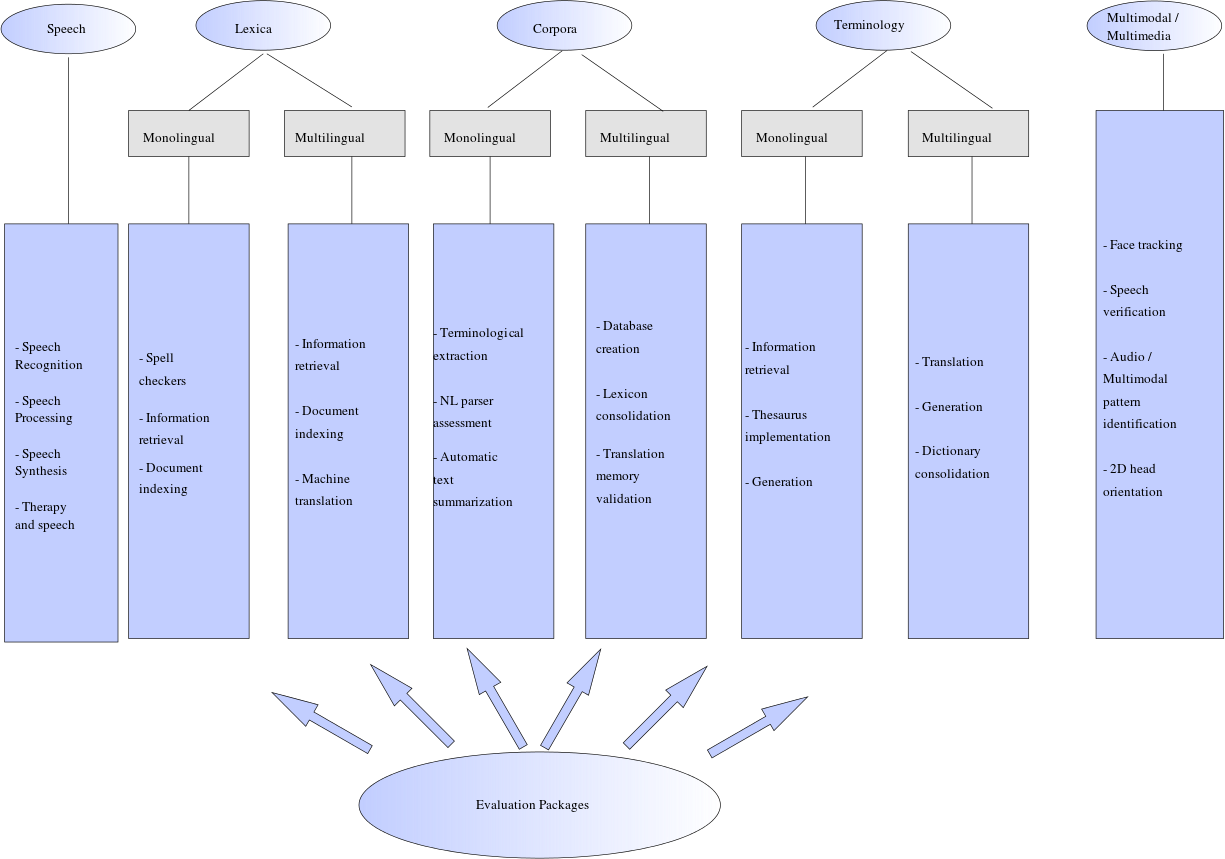
\includegraphics[width=\textwidth]{img/ELRA_supply2.png}

\href{https://catalog.ldc.upenn.edu/byproject}{LDC} (for profit license
27.500\$) provides only NLP related data, especially for language
identification, speech activity detection, speaker recognition, ASR in
english, spanish, arabic, mandarin and many more

\hypertarget{text-based}{%
\subsection{Text-based}\label{text-based}}

\begin{longtable}[]{@{}p{\textwidth/5}p{\textwidth/5}p{\textwidth/5}p{\textwidth/5}p{\textwidth/5}@{}}
\toprule
Name & Purpose & Statistics \& Lables & License & Link\tabularnewline
\midrule
\endhead
Google N-Gram & Corpus (en) & over 8 Mio. books & CC 3.0 &
\href{http://storage.googleapis.com/books/ngrams/books/datasetsv2.html}{Link}\tabularnewline
\bottomrule
\end{longtable}

\hypertarget{visual}{%
\subsection{Visual}\label{visual}}

\hypertarget{object-and-orientationpose-focused-data}{%
\subsubsection{Object and orientation/pose focused
data}\label{object-and-orientationpose-focused-data}}

\begin{longtable}[]{@{}p{\textwidth/5}p{\textwidth/5}p{\textwidth/5}p{\textwidth/5}p{\textwidth/5}@{}}
\toprule
Name & Purpose & Statistics \& Lables & License & Link\tabularnewline
\midrule
\endhead
COCO & Object detection, key point detection, semantic segmentation,
captioning & 128k images with
\href{http://cocodataset.org/\#external}{tons} of labels & CC 4.0 &
\href{http://cocodataset.org/\#overview}{Link}\tabularnewline
Caltech Computer Vision chair data sets & Validation data sets for face
detection and object detection & differs over dataset, below 1000 images
& no license specified &
\href{http://www.vision.caltech.edu/html-files/archive.html}{Link}\tabularnewline
MPII & Human poses and activities & 25k images w 40K people from YouTube
& Simplified BSD &
\href{http://human-pose.mpi-inf.mpg.de/\#overview}{Link}\tabularnewline
SUN database & Object detection \& scene recognition & 108k img, 637
classes scene recognition, 16k imgs object detection & No license
specified &
\href{http://groups.csail.mit.edu/vision/SUN/hierarchy.html}{Link}\tabularnewline
MIT Computational Perception \& Cognition lab & object detection \&
scene recognition & 4 different data sets & no licenses &
\href{http://cvcl.mit.edu/MM/stimuli.html}{Link}\tabularnewline
CIFAR & Object detection & subset of the tiny images dataset, most
widely used benchmark & no license &
\href{http://www.cs.toronto.edu/~kriz/cifar.html}{Link}\tabularnewline
ImageNet & Object detection & 14M images with bounding boxes for 3000
"sysnets" & no license for image urls and annotations &
\href{http://image-net.org/download-imageurls}{Link}\tabularnewline
OpenImages & Object detection & 9M images with 600 classes and bounding
boxes & CC-BY 4.0 &
\href{https://storage.googleapis.com/openimages/web/factsfigures.html}{Link}\tabularnewline
Tiny Images data set & Object detection & 7.5Mio images with 54k nouns
as labels & no license &
\href{http://groups.csail.mit.edu/vision/TinyImages/}{Link}\tabularnewline
ADE20k & Semantic segemntation \& object detection & 22.000 images with
objects and pixel wise segmentation annotations & no license &
\href{http://groups.csail.mit.edu/vision/datasets/ADE20K/}{Link}\tabularnewline
\bottomrule
\end{longtable}

\hypertarget{face-oriented-data}{%
\subsubsection{Face-oriented data}\label{face-oriented-data}}

\begin{longtable}[]{@{}p{\textwidth/5}p{\textwidth/5}p{\textwidth/5}p{\textwidth/5}p{\textwidth/5}@{}}
\toprule
Name & Purpose & Statistics \& Lables & License & Link\tabularnewline
\midrule
\endhead
Helen & Facial landmarks & 2300 images from Flickr & None specified &
\href{http://www.ifp.illinois.edu/~vuongle2/helen/}{Link}\tabularnewline
LFW & Face detection & 5171 faces in 2845 images taken from LFW & None
specified & \href{http://vis-www.cs.umass.edu/lfw/}{Link}\tabularnewline
LFW-a & Face detection & as LFW with improved alignment & None specified
&
\href{https://talhassner.github.io/home/projects/lfwa/index.html}{Link}\tabularnewline
FDDB & Face detection & 13k images with 6k people & None specified &
\href{http://vis-www.cs.umass.edu/fddb/}{Link}\tabularnewline
CUHK Face Alignment db & Face alignment & 13k images from LFW and the
web & None Specified &
\href{http://mmlab.ie.cuhk.edu.hk/archive/CNN_FacePoint.htm}{Link}\tabularnewline
MEDS & Face Detection & ? & none spec &
\href{https://www.nist.gov/itl/iad/image-group/special-database-32-multiple-encounter-dataset-meds}{Link}\tabularnewline
MID & Face Detection & 3248 images, 1573 individuals & None Specified &
\href{https://www.nist.gov/srd/nist-special-database-18}{Link}\tabularnewline
FERET & Face Recognition & ? & custom, free for commercial use &
\href{https://www.nist.gov/itl/iad/image-group/color-feret-database}{Link}\tabularnewline
FIVE & Face detection & ? & ? &
\href{https://www.nist.gov/programs-projects/face-video-evaluation-five}{Link}\tabularnewline
WiderFace & Face recognition & 23k images with 300k faces & None
specified &
\href{http://mmlab.ie.cuhk.edu.hk/projects/WIDERFace/}{Link}\tabularnewline
VisAge & Age and gender classification & Bounding boxes, emotion,
landmark, gender, yaw, pitch, roll, glasses,... currenly 4000 images &
CC 4.0 &
\href{https://www.forensicsandsecurity.com/visage.php}{Link}\tabularnewline
Kaggle challenge & age, emotion, ethnicity & ? & non specified &
\href{https://www.kaggle.com/dataturks/face-dataset-with-age-emotion-ethnicity}{Link}\tabularnewline
FER+ & emotion detection & 35k images & MIT &
\href{https://github.com/Microsoft/FERPlus}{Link}\tabularnewline
VGGFace 2 & face recognition & 9000 ids, 3.3 mio faces & CC share-alike
&
\href{http://www.robots.ox.ac.uk/~vgg/data/vgg_face2/}{Link}\tabularnewline
Multi-Pie \& FiA & landmarks & over 500 GB of high resolution, high
variance images & prorietary (1250\$) &
\href{https://flintbox.com/public/project/5486/}{Link}\tabularnewline
Georgia Face Database & Face detection (validation) & 50 individuals,
with 15 images each, identity and bounding boxes & No license spec. &
\href{http://www.anefian.com/research/face_reco.htm}{Link}\tabularnewline
Youtube Faces DB & Face recognition & 3425 videos of 1600 people with an
average of 181 frames per video & On Request &
\href{http://www.cs.tau.ac.il/~wolf/ytfaces/}{Link}\tabularnewline
IMFDB & age, pose, gender, expression, occulsion & 34512 images of 100
indian actors & None specified &
\href{http://cvit.iiit.ac.in/projects/IMFDB/}{Link}\tabularnewline
Multimodal 3D Faces and emotions & emotions (multiple datasets w diff.
annotations) & depending up to several thousand 3D scans & on request &
\href{http://www.cs.binghamton.edu/~lijun/Research/3DFE/3DFE_Analysis.html}{Link}\tabularnewline
\bottomrule
\end{longtable}

\hypertarget{auditive}{%
\subsection{Auditive}\label{auditive}}

\begin{longtable}[]{@{}p{\textwidth/5}p{\textwidth/5}p{\textwidth/5}p{\textwidth/5}p{\textwidth/5}@{}}
\toprule
Name & Purpose & Statistics \& Lables & License & Link\tabularnewline
\midrule
\endhead
Audioset & Sound vocabulary & 632 audio event classes, 2M human-labeled,
10s clips from YouTube & CC share-alike &
\href{https://research.google.com/audioset/index.html}{Link}\tabularnewline
LibriSpeech & speech corpus (en) & 1000 hours of english speech (audio
books) & CC-BY 4.0 & \href{http://openslr.org/12/}{Link}\tabularnewline
LibriVox & speech corpus (en) & 12000 audio books with transcript & CC0
&
\href{https://librivox.org/search?primary_key=0\&search_category=genre\&search_page=1\&search_form=get_results}{Link}\tabularnewline
Stanford Natural language inference & Sentences and human labeled
judgement (neutral, entailment, contradiction), hypotheses on those
sentences & 570k sentences & CC-BY-SA 4.0 &
\href{https://nlp.stanford.edu/projects/snli/}{Link}\tabularnewline
Stanford Sentiment analysis & sentiment analysis & 240k sentences with 0
to 1 scaled valence (very negative is 0 to very positive is 1) & None
specified &
\href{https://nlp.stanford.edu/sentiment/code.html}{Link}\tabularnewline
Voices & noise cancellation, speech recognition, speaker recognition,
... & 200 speakers, 15 hours & CC-BY 4.0 &
\href{https://voices18.github.io/}{Link}\tabularnewline
SpokenLanguages2 & Spoken language identification & 66k, 10s mp3
sequences and the language label &
\href{https://community.topcoder.com/longcontest/?module=ViewProblemStatement\&rd=16555\&pm=13978}{Link}
&\tabularnewline
EmoV-DB & Emotional speeech synthesis and classification & 4.1k and were
downsampled at 16k and stored in 16-bit PCM WAV format, 5 speakers with
over 500 utterances each & none specified &
\href{http://www.coe.neu.edu/Research/AClab/Speech\%20Data/}{Link}\tabularnewline
\bottomrule
\end{longtable}

\hypertarget{audio-visual}{%
\subsection{Audio-Visual}\label{audio-visual}}

\begin{longtable}[]{@{}p{\textwidth/5}p{\textwidth/5}p{\textwidth/5}p{\textwidth/5}p{\textwidth/5}@{}}
\toprule
Name & Purpose & Statistics \& Lables & License & Link\tabularnewline
\midrule
\endhead
AVSpeech & Speeker Separation & 290k, 3-10s YouTube videos w no
background noise and a single speaker & CC 4.0 &
\href{https://looking-to-listen.github.io/avspeech/index.html}{Link}\tabularnewline
EmoVoxCeleb & modality-transferring emotion detection & identity,
emotion labels for images & CC share-alike &
\href{http://www.robots.ox.ac.uk/~vgg/research/cross-modal-emotions/}{Link}\tabularnewline
VoxCeleb & Emotion detection, speaker ID, Speech separation & 7000
Speakers, 1mio utterances, 2000 hours & CC share-alike &
\href{http://www.robots.ox.ac.uk/~vgg/data/voxceleb/index.html\#portfolio}{Link}\tabularnewline
VGGLip & Lip reading, speech separation, speech recognition & 6M word
instances, 800 hours, 5000 identities & CC-share-alike &
\href{http://www.robots.ox.ac.uk/~vgg/data/lip_reading/}{Link}\tabularnewline
\bottomrule
\end{longtable}